
\section{Population subdivision}

\begin{frame}{Intended Learning Outcomes}

	\underline{Population subdivision}

	\bigskip

	In this lecture you will learn to
	\begin{itemize}
		\item quantify the effect of population subdivision on allele frequencies and heterozygosity
		\item calculate measures of population genetic differentiation
		\item discuss divergence models
	\end{itemize}

\end{frame}


\begin{frame}{Population subdivision}

	\begin{block}{}
		There is population subdivision, or \textbf{structure}, when the population is not randomly mating
		because of geographic or social structure.
	\end{block}

	\bigskip

	Population subdivision is important to
	\begin{itemize}
		\item understand the effects of drift and natural selection
		\item plan conservation strategies for rare or endangered species
	\end{itemize}

\end{frame}


\begin{frame}{Population subdivision}

        \begin{figure}
                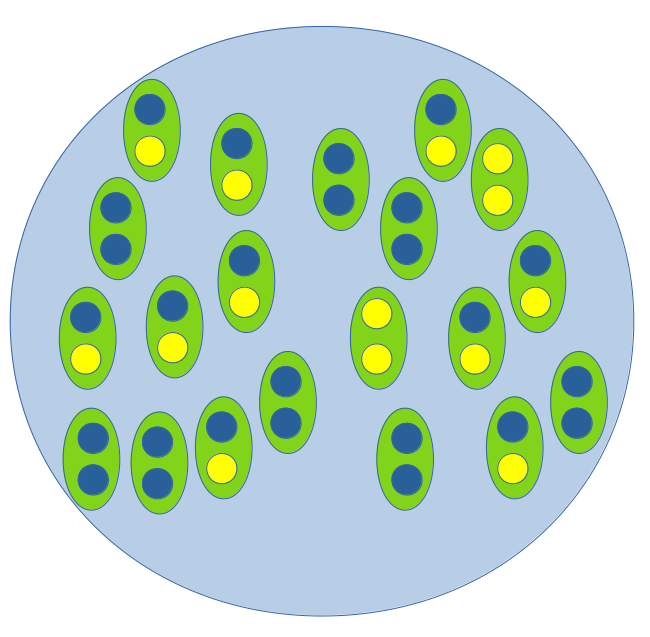
\includegraphics[width=0.65\textwidth]{Pics/predivision}
        \end{figure}

\end{frame}


\begin{frame}{Population subdivision}

	\begin{figure}
                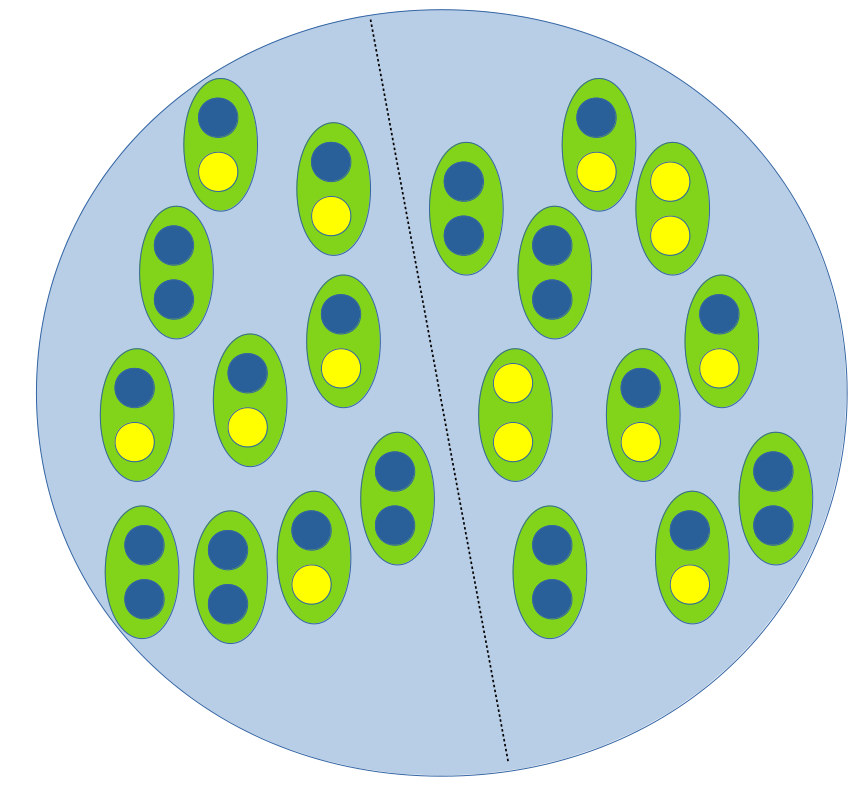
\includegraphics[width=0.65\textwidth]{Pics/division}
        \end{figure}

\end{frame}


\begin{frame}{Allele frequencies in a subdivided population}

        \begin{columns}

                \column{0.3\textwidth}

                \begin{figure}
			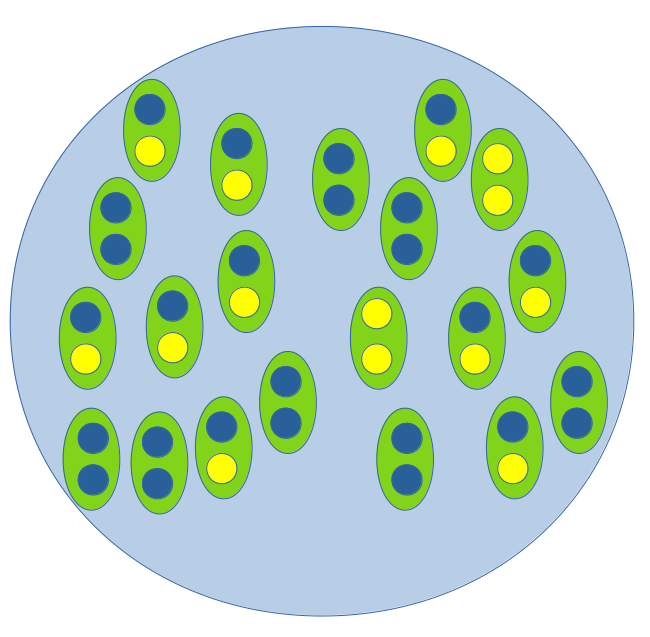
\includegraphics[width=0.8\textwidth]{Pics/predivision} \
                        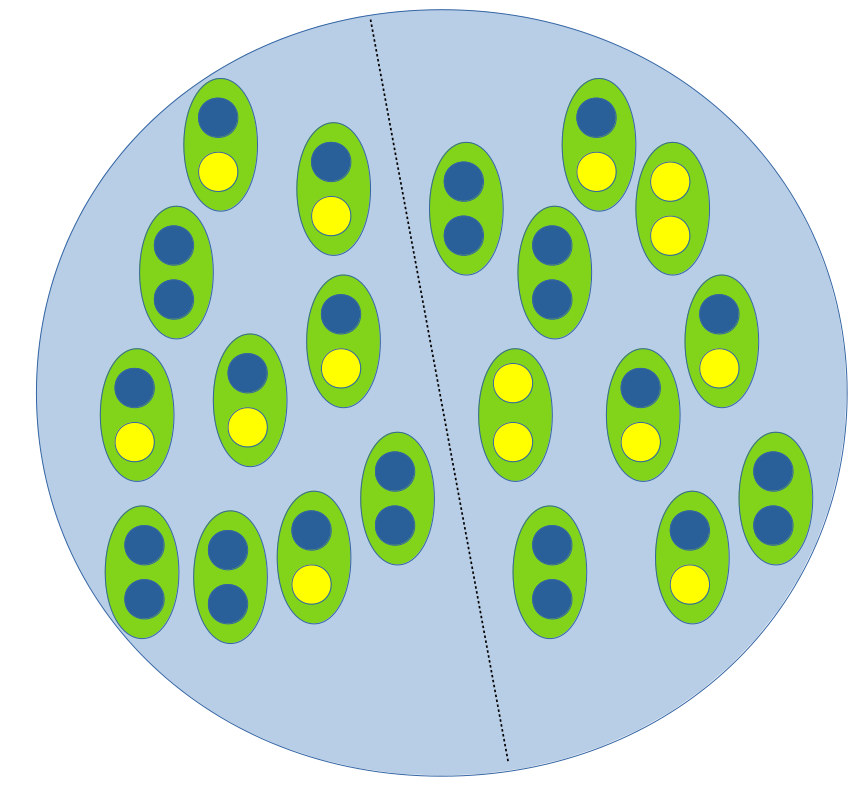
\includegraphics[width=0.8\textwidth]{Pics/division}
                \end{figure}

                \column{0.7\textwidth}

		Assume two subpopulations, each one in HW equilibrium with $N_1$ and $N_2$ individuals, respectively.

		\vskip 0.5cm

		The average frequency of allele $A$ when pooling the two subpopulations is
		\begin{equation}
			f_A = \frac{2 N_1 f_{A1} + 2 N_2 f_{A2}}{2N_1 + 2N_2}
		\end{equation}
		If $N_1=N_2$
		\begin{equation}
                        f_A = \frac{f_{A1} + f_{A2}}{2}
                \end{equation}

        \end{columns}

\end{frame}


\begin{frame}{Heterozygosity in a subdivided population}

        \begin{columns}

                \column{0.3\textwidth}

                \begin{figure}
			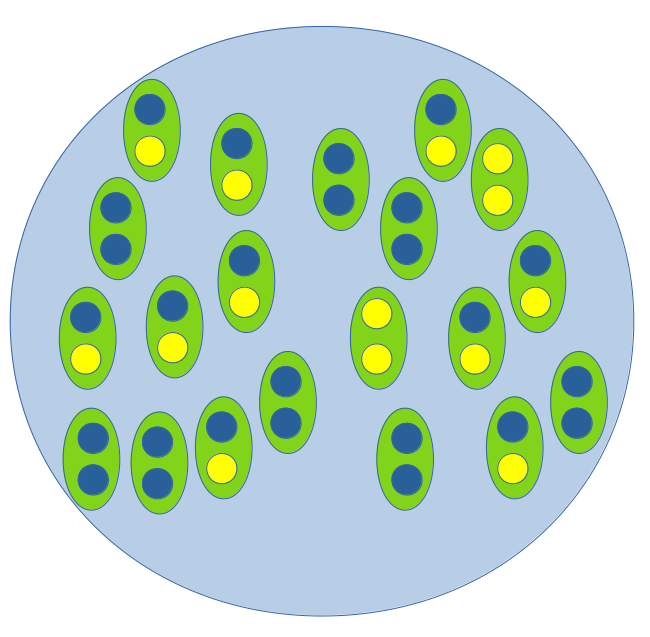
\includegraphics[width=0.8\textwidth]{Pics/predivision} \
                        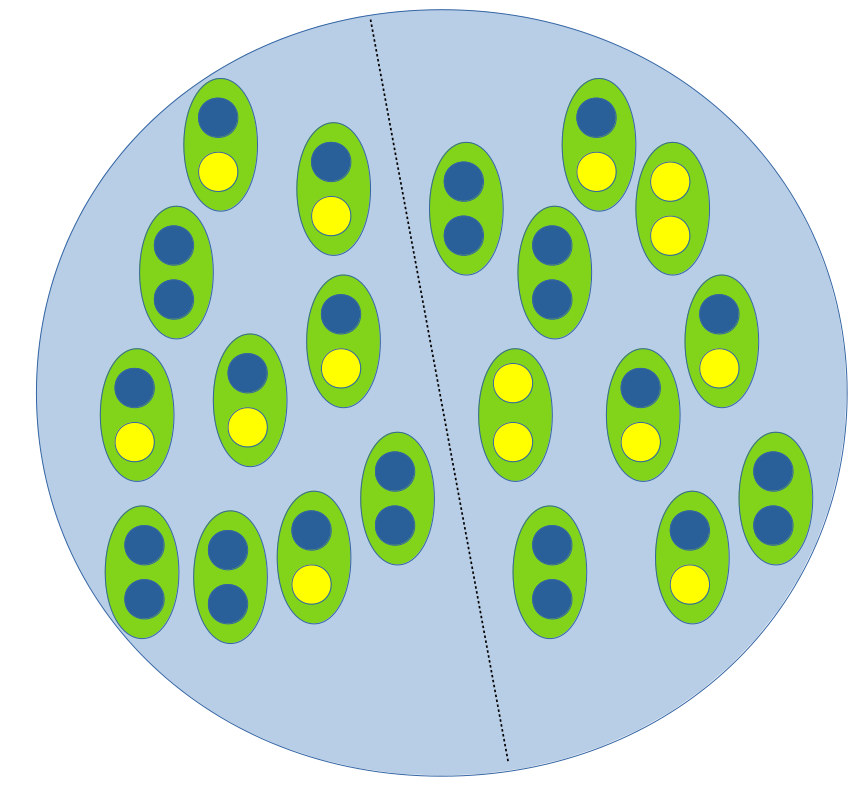
\includegraphics[width=0.8\textwidth]{Pics/division}
                \end{figure}

                \column{0.7\textwidth}

		The proportion of heterozygous individuals is
                \begin{equation}
                        H_S = \frac{2f_{A1}(1-f_{A1}) + 2f_{A2}(1-f_{A2})}{2}
                \end{equation}
		which is the expected heterozygosity when both populations are sampled.

		\bigskip

		\small{$S$ in $H_S$ stands for "in the \underline{s}ubdivided population"}
	
        \end{columns}

\end{frame}


\begin{frame}{Heterozygosity in a subdivided population}

        \begin{columns}

                \column{0.3\textwidth}

                \begin{figure}
			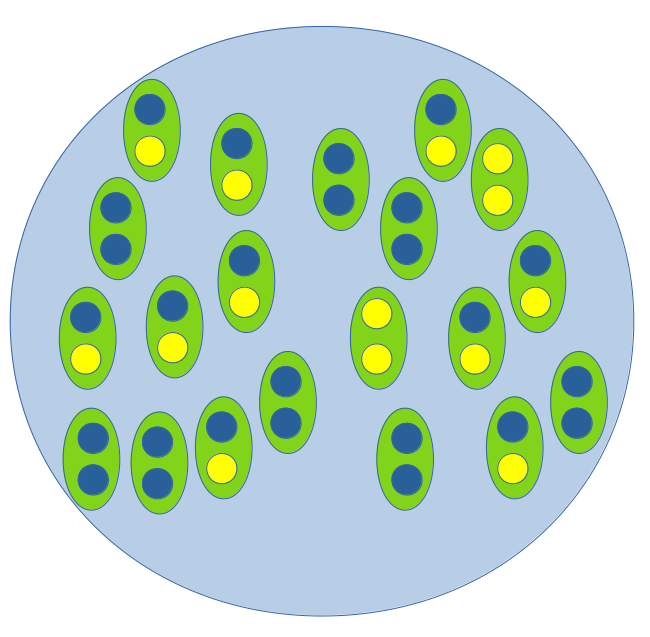
\includegraphics[width=0.8\textwidth]{Pics/predivision} \
                        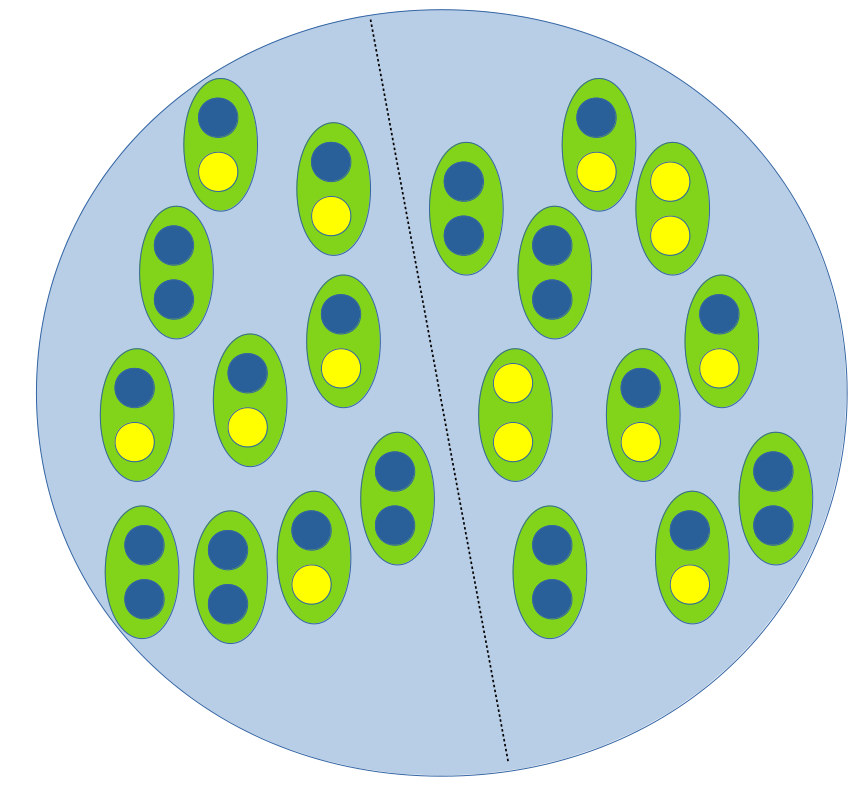
\includegraphics[width=0.8\textwidth]{Pics/division}
                \end{figure}

                \column{0.7\textwidth}

                However, the expected proportion of heterozygous individuals in a population with frequency $f_A$ is
                \begin{equation}
                        H_T = 2 \frac{f_{A1} + f_{A2}}{2} (1 - \frac{f_{A1} + f_{A2}}{2})
                \end{equation}

                \bigskip

                \small{$T$ in $H_T$ stands for "in the \underline{t}otal (pooled) population"}
        
        \end{columns}

\end{frame}


\begin{frame}{Heterozygosity in a subdivided population}

	After some rearrangements we have
	\begin{equation}
		H_S = f_{A1}(1-f_{A1}) + f_{A2}(1-f_{A2})
	\end{equation}
	and
	\begin{equation}
                H_T = f_{A1}(1-f_{A1}) + f_{A2}(1-f_{A2}) + \delta^2/2
        \end{equation}
	with $\delta = |f_{A1}-f_{A2}|$.

\end{frame}


\begin{frame}{Heterozygosity in a subdivided population}

	$H_T = H_S + \delta^2/2$

	\begin{itemize}
		\item If $\delta=0$ then \pause $H_T=H_S$ and the total (pooled) population is also in HWE.
		\item If $\delta>0$ then \pause $H_T<H_S$ and \pause the total (pooled) population contains fewer 
		heterozygous individuals than expected given the pooled allele frequency.
	\end{itemize}

	\begin{block}{Wahlund effect}
		The decrease of heterozygosity in a subdivided population compared to a randomly
		mating one with the same (total) allele frequency.
	\end{block}

\end{frame}


\begin{frame}{Quantifying population subdivision}

	\begin{equation}
		F_{ST} = \frac{H_T - H_S}{H_T}
	\end{equation}

	\pause
	$F_{ST}$ has a range defined as
	\begin{itemize}
		\item if $\delta=0$ then $H_T=H_S$ and $F_{ST}=0$
		\item if $\delta=1$ then $F_{ST}=1$
	\end{itemize}

	\bigskip

	$F_{ST}$ can be calculated for more than two subpopulations.

\end{frame}


\begin{frame}{$F_{ST}$: population genetic differentiation}

	\begin{figure}
        	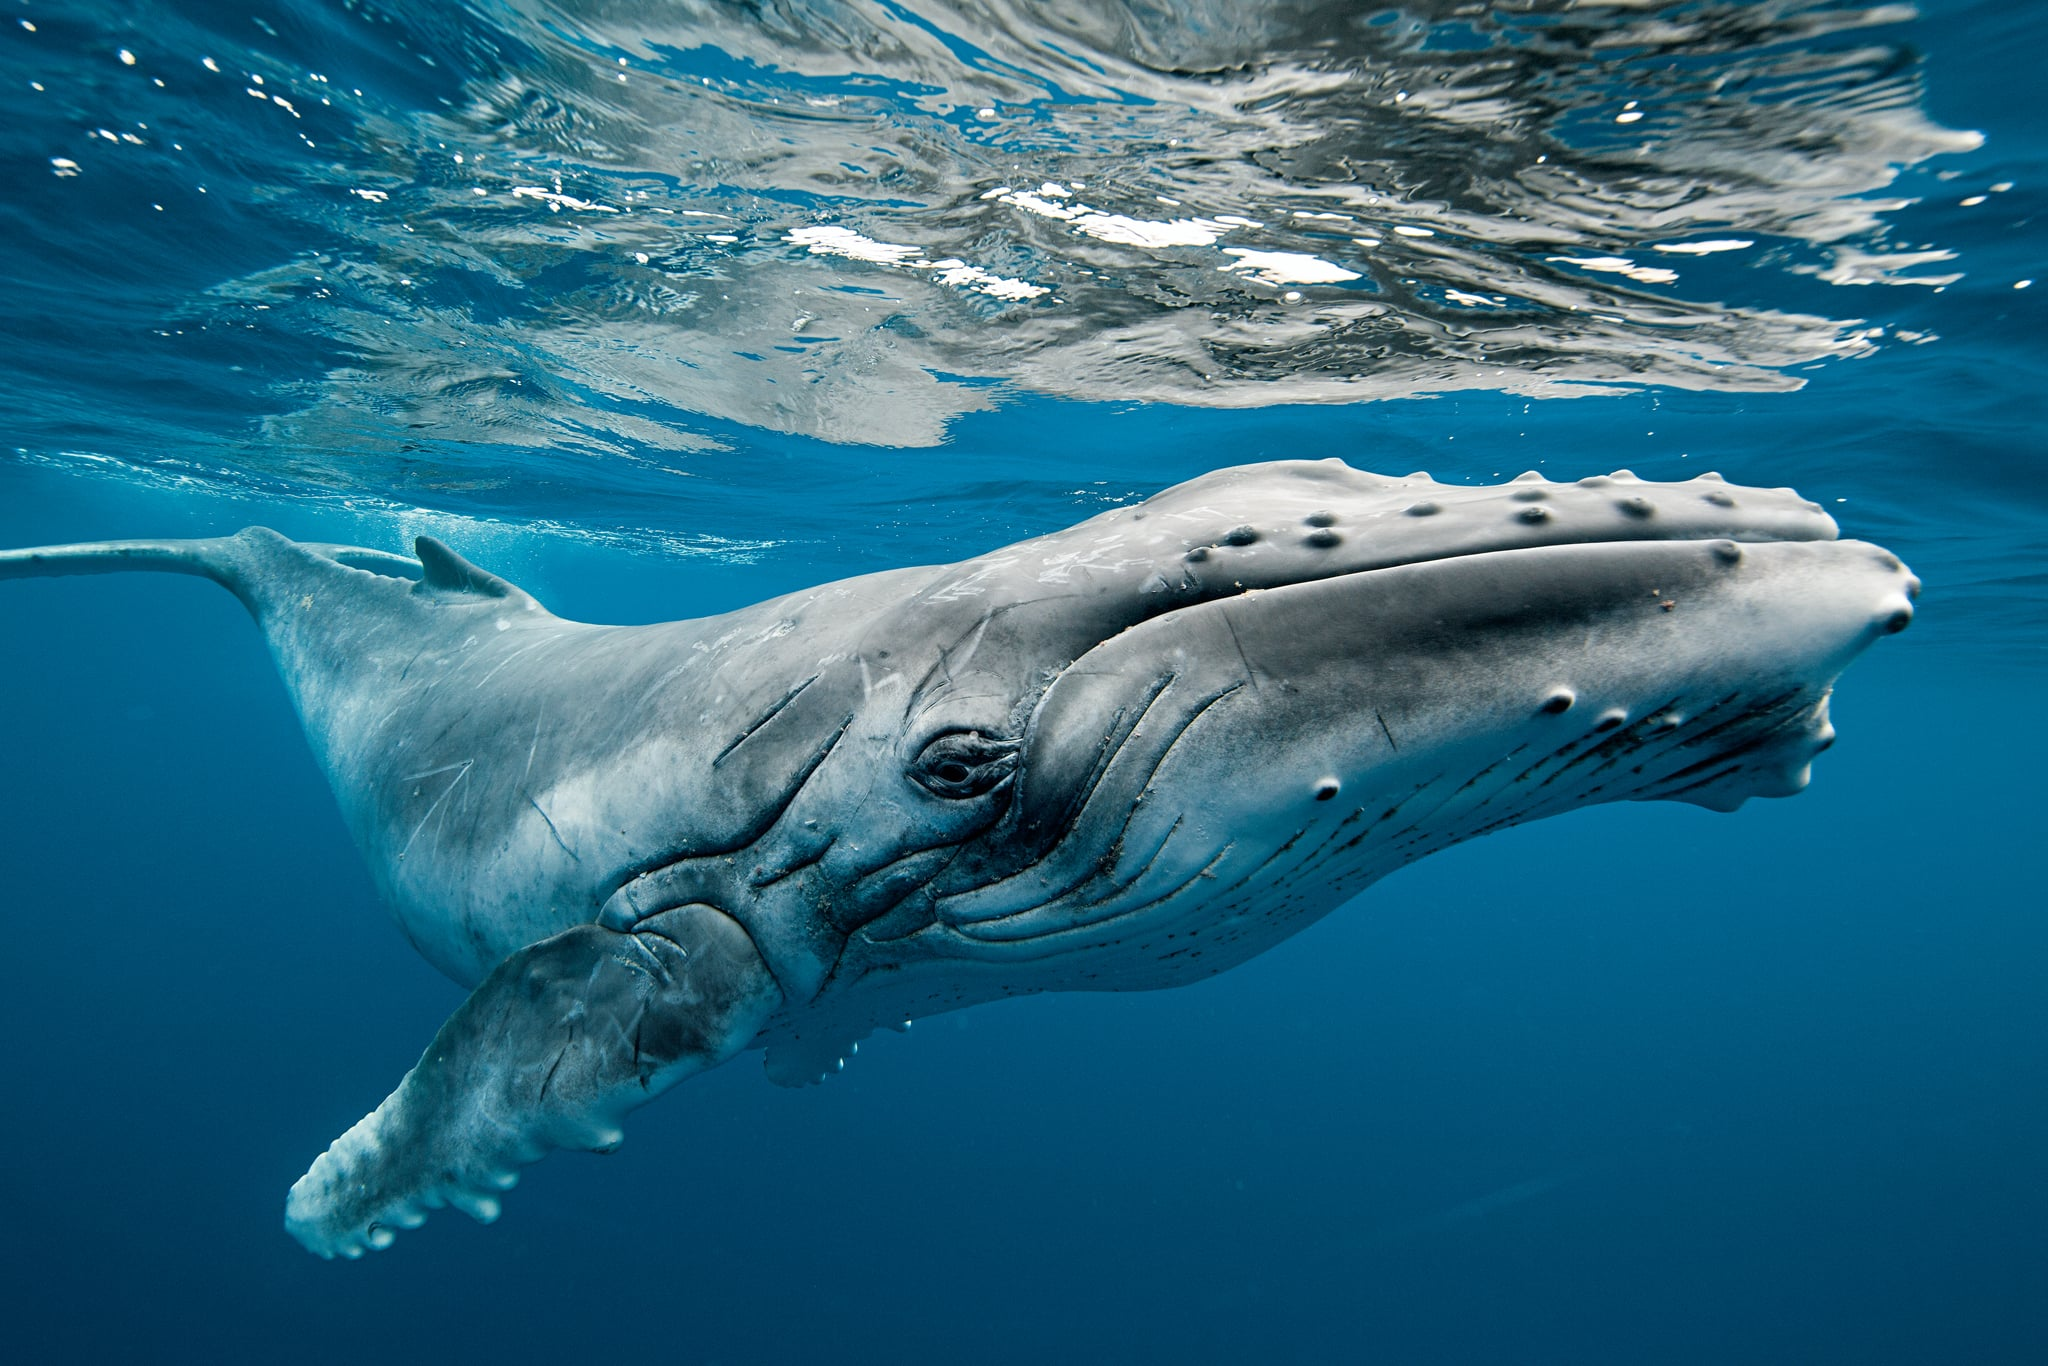
\includegraphics[width=0.5\textwidth]{Pics/whale} \
		\caption{\small Humpback whales in the Pacific and Atlantic have strong genetic differentiation ($F_{ST}>0.4$) while populations in the North Atlantic have low differentation  ($F_{ST} \approx 0.04$).}
        \end{figure}

\end{frame}


\begin{frame}{Wright-Fisher model with migration}

        \begin{figure}
                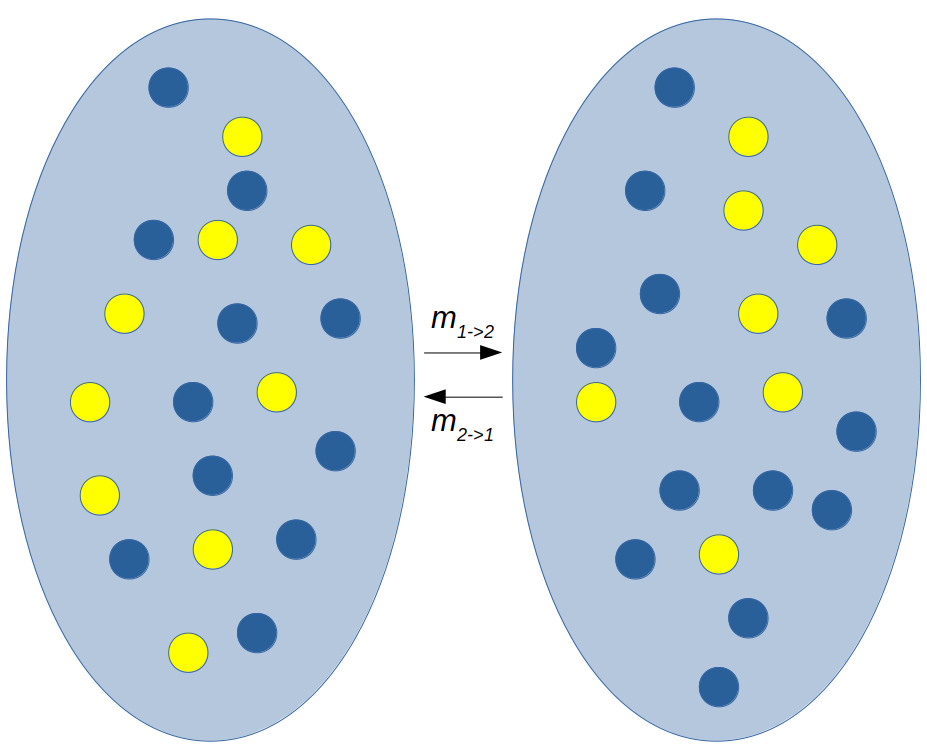
\includegraphics[width=0.6\textwidth]{Pics/migration} \
                \caption{\small An individual from one population is replaced with an individual from the other with probability $m$ (migration rate).}
        \end{figure}

\end{frame}


\begin{frame}{$F_{ST}$ and migration rates}

	Using the coalescence theory assuming an infinite sites model, we can derive that
	\begin{equation}
		F_{ST} = \frac{1}{1 + 4Nm_T}
	\end{equation}
	with $m_T$ being the total number of migrants.

	\bigskip
	\tiny jupyter-notebook: subdivision

\end{frame}


\begin{frame}{"Island" model}

	\small
	\begin{block}{}
	It assumes that populations have been subdivided for a very long time so that 
	an equilibrium has been established and that then there is ongoing \textbf{gene-flow}.
	\end{block}
	It is not a realistic model for some species.

	\pause
	\begin{figure}
                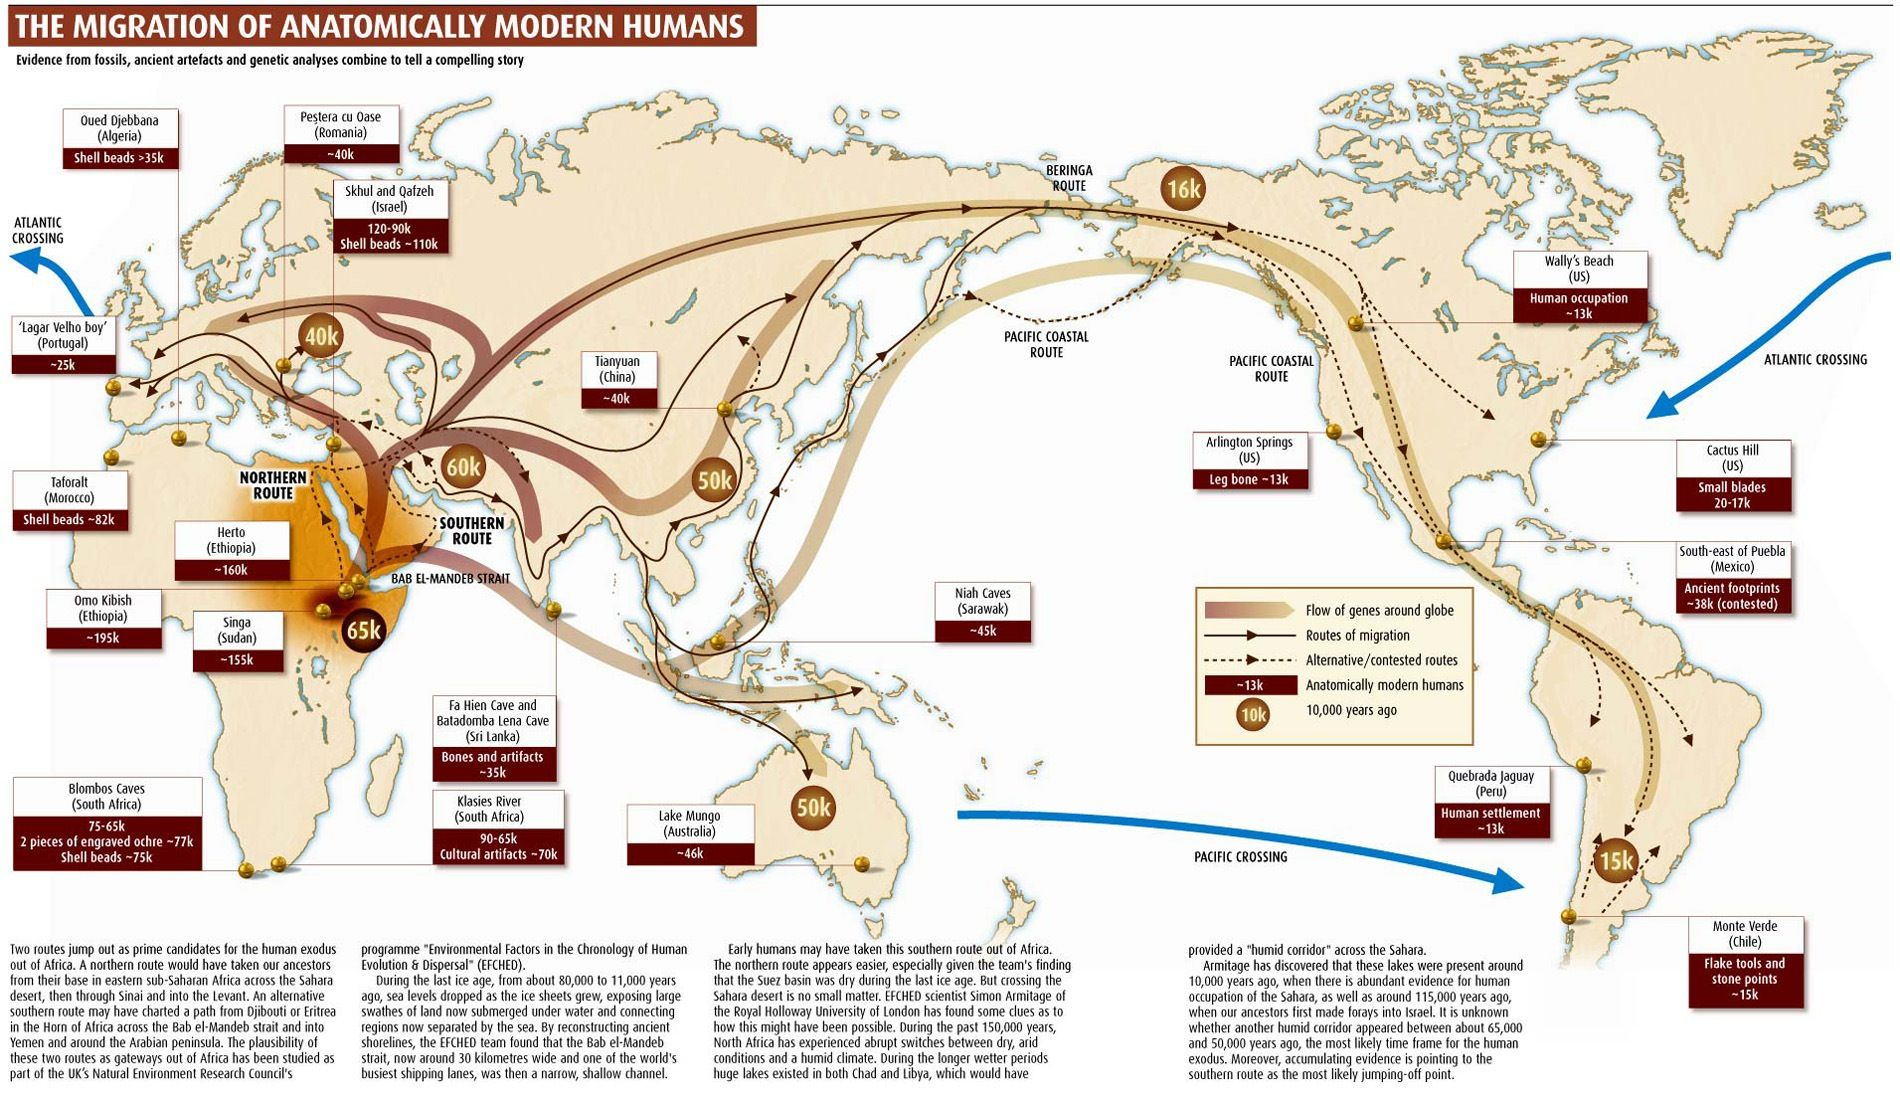
\includegraphics[width=0.6\textwidth]{Pics/human_evo}
        \end{figure}


\end{frame}


\begin{frame}{Divergence model}

	\small
	\begin{block}{}
		It describes populations diverging from common ancestral populations without subsequent gene-flow.
	\end{block}

	\begin{figure}
                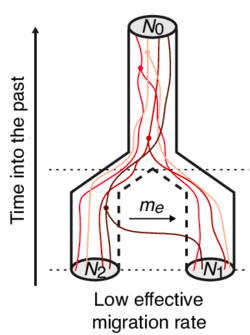
\includegraphics[width=0.3\textwidth]{Pics/coal_divergence} \
		\caption{\small TMRCA overestimates the divergence time.}
        \end{figure}

\end{frame}


\begin{frame}{Isolation by distance}

	\begin{block}{}
		The degree of population subdivision increases with geographical distance.
	\end{block}

	\bigskip

	\begin{itemize}
		\item migration rate is a linear function of geographical distance
		\item migration occurs only between adjacent populations (stepping-stone models)
		\item series of divergence events (sequential colonisation)
	\end{itemize}

\end{frame}

\begin{frame}{Isolation by distance}

	\begin{figure}
                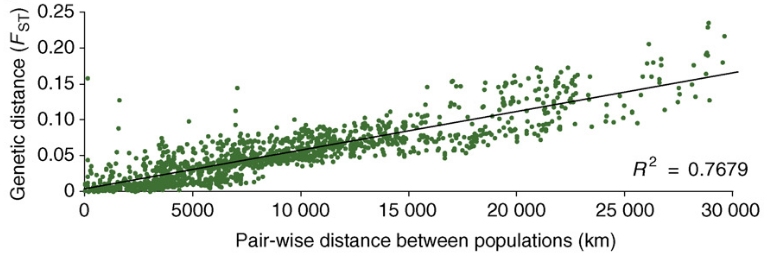
\includegraphics[width=0.9\textwidth]{Pics/handley} \
                \caption{\small Isolation by distance in human populations.}
        \end{figure}

\end{frame}


\begin{frame}{Intended Learning Outcomes}

        \underline{Population subdivision}

        \bigskip

        In this lecture you have learned to
        \begin{itemize}
                \item quantify the effect of population subdivision on allele frequencies and heterozygosity
                \item calculate measures of population genetic differentiation
                \item discuss divergence models
        \end{itemize}

\end{frame}


